\documentclass[shownotes,11pt, aspectratio=169]{beamer}

\usepackage{pgfpages}
% These slides also contain speaker notes. You can print just the slides,
% just the notes, or both, depending on the setting below. Comment out the want
% you want.
\setbeameroption{hide notes} % Only slide
%\setbeameroption{show only notes} % Only notes
%\setbeameroption{show notes on second screen=right} % Both

\usepackage{helvet}
\usepackage[default]{Fira Sans}
\usepackage{array}
\usepackage{caption}
%\usepackage[clean]{svg}
\usepackage{tikz}
\usepackage{verbatim}
\setbeamertemplate{note page}{\pagecolor{yellow!5}\insertnote}
\usetikzlibrary{positioning}
\usetikzlibrary{snakes}
\usetikzlibrary{calc}
\usetikzlibrary{arrows}
\usetikzlibrary{decorations.markings}
\usetikzlibrary{shapes.misc}
\usetikzlibrary{matrix,shapes,arrows,fit,tikzmark}
\usepackage{amsmath}
\usepackage{mathpazo}
\usepackage{hyperref}
\usepackage{lipsum}
\usepackage{multimedia}
\usepackage{graphicx}
\usepackage{multirow}
\usepackage{graphicx}
\usepackage{dcolumn}
\usepackage{bbm}
\usepackage{tfrupee}
\newcolumntype{d}[0]{D{.}{.}{5}}

\usepackage{changepage}
\usepackage{appendixnumberbeamer}
\newcommand{\beginbackup}{
   \newcounter{framenumbervorappendix}
   \setcounter{framenumbervorappendix}{\value{framenumber}}
   \setbeamertemplate{footline}
   {
     \leavevmode%
     \hline
     box{%
       \begin{beamercolorbox}[wd=\paperwidth,ht=2.25ex,dp=1ex,right]{footlinecolor}%
%         \insertframenumber  \hspace*{2ex} 
       \end{beamercolorbox}}%
     \vskip0pt%
   }
 }
\newcommand{\backupend}{
   \addtocounter{framenumbervorappendix}{-\value{framenumber}}
   \addtocounter{framenumber}{\value{framenumbervorappendix}} 
}


\usepackage{graphicx}
\usepackage[space]{grffile}
\usepackage{booktabs}

% These are my colors -- there are many like them, but these ones are mine.
\definecolor{blue}{RGB}{0,114,178}
\definecolor{red}{RGB}{213,94,0}
\definecolor{yellow}{RGB}{240,228,66}
\definecolor{green}{RGB}{0,158,115}

\hypersetup{
  colorlinks=false,
  bookmarks=true,
  linkbordercolor = {white},
  linkcolor = {blue}
}


%% I use a beige off white for my background
\definecolor{MyBackground}{RGB}{255,253,218}

%% Uncomment this if you want to change the background color to something else
\setbeamercolor{background canvas}{bg=MyBackground}

%% Change the bg color to adjust your transition slide background color!
\newenvironment{transitionframe}{
  \setbeamercolor{background canvas}{bg=yellow}
  \begin{frame}}{
    \end{frame}
}

\setbeamercolor{frametitle}{fg=blue}
\setbeamercolor{title}{fg=black}
\setbeamertemplate{footline}[frame number]
\setbeamertemplate{navigation symbols}{} 
\setbeamertemplate{itemize items}{-}
\setbeamercolor{itemize item}{fg=blue}
\setbeamercolor{itemize subitem}{fg=blue}
\setbeamercolor{enumerate item}{fg=blue}
\setbeamercolor{enumerate subitem}{fg=blue}
\setbeamercolor{button}{bg=MyBackground,fg=blue,}



% If you like road maps, rather than having clutter at the top, have a roadmap show up at the end of each section 
% (and after your introduction)
% Uncomment this is if you want the roadmap!
% \AtBeginSection[]
% {
%    \begin{frame}
%        \frametitle{Roadmap of Talk}
%        \tableofcontents[currentsection]
%    \end{frame}
% }
\setbeamercolor{section in toc}{fg=blue}
\setbeamercolor{subsection in toc}{fg=red}
\setbeamersize{text margin left=1em,text margin right=1em} 

\newenvironment{wideitemize}{\itemize\addtolength{\itemsep}{10pt}}{\enditemize}

\title[]{\textcolor{blue}{Macroeconomics: Lecture 5}}
\author[SM]{Sumit Mishra}
\institute[IFMR]{\small{\begin{tabular}{c}
IFMR, Sri City \\
\end{tabular}}}

\date{03 October, 2019}


\begin{document}

%%% TIKZ STUFF
\tikzset{   
        every picture/.style={remember picture,baseline},
        every node/.style={anchor=base,align=center,outer sep=1.5pt},
        every path/.style={thick},
        }
\newcommand\marktopleft[1]{%
    \tikz[overlay,remember picture] 
        \node (marker-#1-a) at (-.3em,.3em) {};%
}
\newcommand\markbottomright[2]{%
    \tikz[overlay,remember picture] 
        \node (marker-#1-b) at (0em,0em) {};%
}
\tikzstyle{every picture}+=[remember picture] 
\tikzstyle{mybox} =[draw=black, very thick, rectangle, inner sep=10pt, inner ysep=20pt]
\tikzstyle{fancytitle} =[draw=black,fill=red, text=white]
%%%% END TIKZ STUFF

% Title Slide
\begin{frame}
\maketitle
%  \centering The views expressed do not necessarily reflect the position of the Federal Reserve Bank of New York or the Federal Reserve System.
\end{frame}

%%SLIDE 1
\begin{frame}
\frametitle{Agenda}
\begin{itemize}
\item Overview of the labour market.
\item Unemployment rate, and its effects.
\item Wage and price determination.
\item Natural rate of unemployment.
\item Material: Blanchard, Chapter 6.
\end{itemize}
\end{frame}

\section{Basic Facts About Indian Labour Market}
\begin{frame}{Labour Force Participation Rate}
\begin{center}
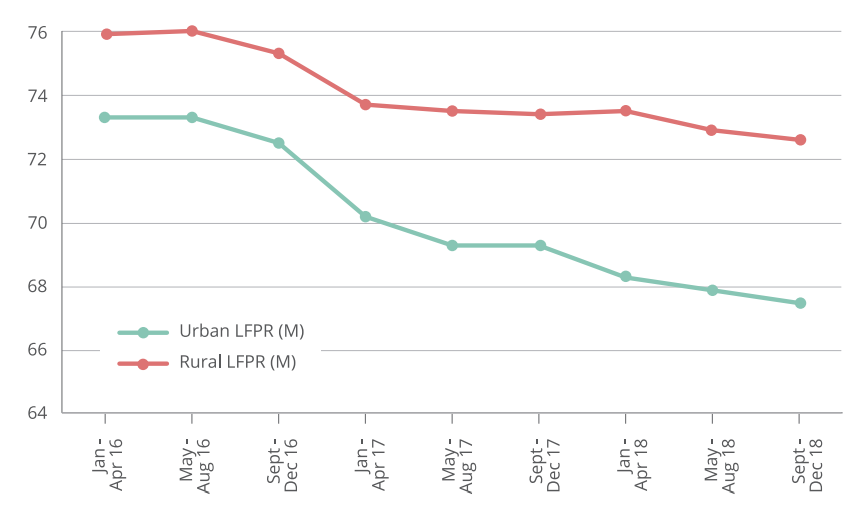
\includegraphics[scale=0.5]{graphs/L052019F01.png}
\footnote{Source: \url{https://cse.azimpremjiuniversity.edu.in/wp-content/uploads/2019/04/SWI2019_Employment_Trends.pdf}}
\end{center}
\end{frame}

\begin{frame}{Unemployment in India: Last Two Decades}
\begin{center}
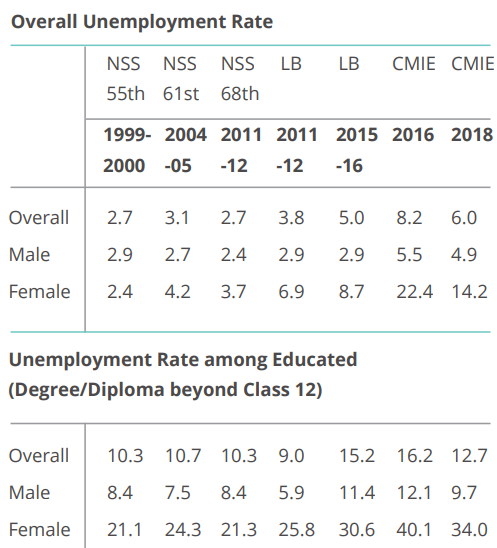
\includegraphics[scale=0.5]{graphs/L052019F02.png}
\end{center}
\end{frame}

%%%%%%%%%%%%%%%%%%%%%%%%%%%%%%%%%%%%%%%%%%%%%%%%%%%%
\section{Unemployment and Worker}
\begin{frame}{Unemployment and Worker}
How do fluctuations in \textit{unemployment rate} affect \textit{individual workers}?
\begin{itemize}
\item It matters for the welfare of individual workers.
\item It determines \pause wages.
\end{itemize}
\pause
What do firms do when there is fall in demand? \pause
\\
\textcolor{red}{They can stop hiring new people.}
\end{frame}

\begin{frame}{Unemployment and Worker}
What implications does this movement have for the workers?
\begin{wideitemize}
\item If the adjustment happens via hiring stoppage, finding a job might be tough.
\item If the adjustment happens via firing, the odds of losing a job become higher.
\end{wideitemize}
\end{frame}

\section{Wage Determination}
%%%%%%%%%%%%%%%%%%%%%%%%%%%%%%%%%%%%%%%%%%%%%%%%%%%%%%%%%%
\begin{frame}
\frametitle{Wage Determination}
\begin{wideitemize}
\item Let me hear you out on this first.
\pause
\item Wages are \textbf{NOT} typically determined by supply and demand.
\pause
\item Wages are determined by bargaining between the firm and the labour union/the employee.
\item The bargaining will be harder for \pause the jobs that require better skills.
\pause
\item \textit{Workers are typically paid a wage that exceeds their reservation wage, the wage
that would make them indifferent between working or being unemployed.}
\end{wideitemize}
\end{frame}

\begin{frame}
\frametitle{Bargaining}
Bargaining depends on two variables--
\begin{itemize}
\item[1] Cost that a firm would incur when the employee leaves.
\item[2] How easy is it for the employee to find another job?
\end{itemize}
\pause
\textbf{Implications}
\begin{itemize}
\item[1] \textcolor{red}{Skills fetch worker greater bargaining power.}
\item[2] \textcolor{red}{Labour market conditions determine bargaining power.}
\end{itemize}
\end{frame}

\begin{frame}
\frametitle{Efficiency Wages}
Firms may want to pay more than the `reservation' wage. \pause
Reason: \textbf{Incentivizes productivity}.
\\
\vspace{3mm}
Firms want their workers to feel good about their jobs. This is \textbf{efficiency wage theory} in nutshell.
\\
\vspace{3mm}
Wages, once again, depend upon the type of job and labour market conditions. 
\end{frame}

%%%%%%%%%%%%%%%%%%%%%%%%%%%%%%%%%%%%%
\section{Wages, Prices, and Unemployment}
\begin{frame}
\[ W = P^eF(u, z) \]
The nominal wage $W$ depends upon three variables:
\begin{itemize}
\item The expected price level $P^e$.
\item The unemployment rate $u$
\item All other variables indexed as $z$.
\end{itemize}
\end{frame}

\begin{frame}{The Expected Price Level}
\begin{wideitemize}
\item All involved- firms as well as workers- care about \textbf{real wages}.
\item Workers care about what they can buy with the wages.
\item Firms care about the price of the good ($P$) and the wages relative to these prices.
\item Typically, actual price level is not known in advance. So, workers form expectations about the price level.
\end{wideitemize}
\end{frame}

\begin{frame}{The Unemployment Rate}
\begin{itemize}
\item Higher unemployment rate weakens \pause worker's bargaining power.
\pause
\item Therefore, unemployment rate and wages are inversely related in our model.
\end{itemize}
\end{frame}

\begin{frame}{Other Factors}
A very long list. I would first hear your view on this.
\pause
\begin{wideitemize}
\item \textbf{Unemployment Insurance}: \textit{At a given unemployment rate, higher unemployment benefits
increase the wage.}
\item \textbf{Employment Protection}: This makes hiring new workers or firing the existing ones a costly affair. Worker's bargaining power goes up. Therefore, the average wage would go up as well.
\item What if minimum wage shifts?
\end{wideitemize}
\end{frame}

%%%%%%%%%%%%%%%%%%%%%%%%%%%%%%%%%%%%%%%%%%%%%%%%%%%%%%%%%%
\section{Price Determination}
\begin{frame}{Price Determination}
\begin{itemize}
\item We know from microeconomics that the price is a function of costs. 
\item We also know from microeconomics that costs depend upon the type of production function.
\item At this point, we just simplify everything:
     \[ Y = AN \]
\item $Y$ is output, $N$ is labour, $A$ is some estimated measure of productivity.
\item One more (over)simplification: $A = 1$.
\item What's the marginal cost here? \pause $W$
\item In perfect competition: $P = MR = MC$.
\item But not all firms in our toy economy are competitive. 
\end{itemize}
\end{frame}

\begin{frame}{Price Determination}
\begin{wideitemize}
\item Some firms enjoy markup. ($m$)
\item So, in aggregate, 
     \[ P = (1 + m)W \]
\item Had economy been populated with perfectly competitive firms, what would be the price level? \pause
     \[ P = W \]
\end{wideitemize}
\end{frame}

\section{The Natural Rate of Unemployment}
\begin{frame}{The Wage Setting Relation}
Rewind to.. \pause
\[ W = PF(u,z) \] 
\pause
Rework this equation to get: 
\[ \frac{W}{P} = F(u,z) \]
\end{frame}

\begin{frame}{The Price Setting Relation}
We learnt that
\[ P = (1 + m)W \]
Rearrange this equation such that:
\[ \frac{W}{P} = \frac{1}{(1 + m)} \]
How do we translate this equation into English? Help! \pause
\begin{itemize}
\item Real wage depends upon firms' markup price.
\item \textit{An increase in the markup leads firms to increase their prices given the wage
they have to pay.} \pause
\item Therefore, the real wages should fall. 
\end{itemize}
\end{frame}

\begin{frame}
\makebox[\linewidth][c]{
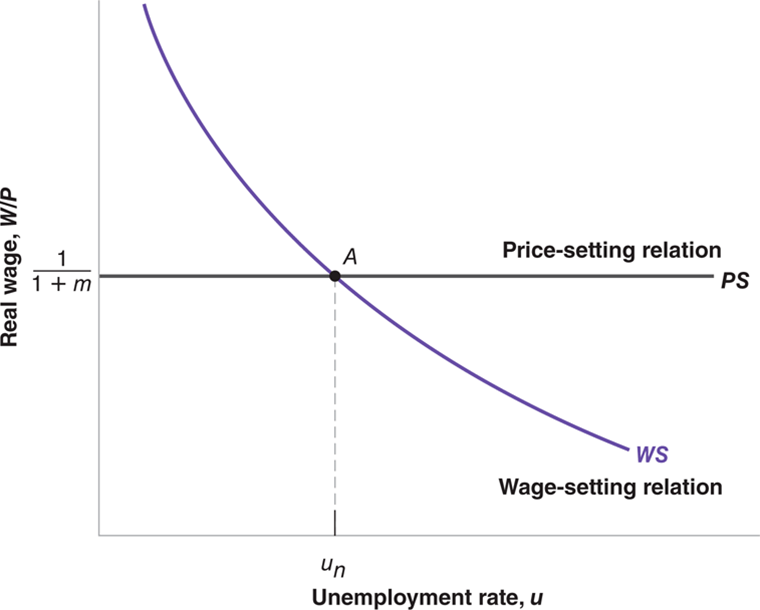
\includegraphics[scale=0.72]{graphs/L5F1.png}}
\end{frame}

\begin{frame}{Equilibrium}
\begin{wideitemize}
\item Equilibrium in the labour market: real wage chosen in wage setting = real wage determined by price setting.
\item We can bring in the relationship between real wages and unemployment now. 
     \[ F(u_n, z) = \frac{1}{1 + m} \]
\item The equilibrium unemployment rate is known as the \textcolor{red}{natural rate of unemployment}.
\item $u_n$ depends upon $m, z$.
\end{wideitemize}
\end{frame}

\begin{frame}{Natural Rate of Unemployment: Nothing Natural About It}
\begin{wideitemize}
\item Equilibrium in the labour market: real wage chosen in wage setting = real wage determined by price setting.
\item We can bring in the relationship between real wages and unemployment now. 
     \[ F(u_n, z) = \frac{1}{1 + m} \]
\item The equilibrium unemployment rate is known as the \textcolor{red}{natural rate of unemployment}.
\item $u_n$ depends upon $m, z$.
\end{wideitemize}
\end{frame}

\begin{frame}
\begin{wideitemize}
\item Suppose there is a rise in unemployment benefits. This shifts the wages upwards.
\pause
\item \textcolor{red}{$\uparrow$ unemployment benefits $\Rightarrow$ $\uparrow$ real wage}.
\pause
\item Poor enforcement of anti-competition policies. \pause 
\item \textcolor{red}{$\uparrow$ markup $\Rightarrow$ $\downarrow$ real wage.}
\end{wideitemize}
\end{frame}

\begin{frame}
\makebox[\linewidth][c]{
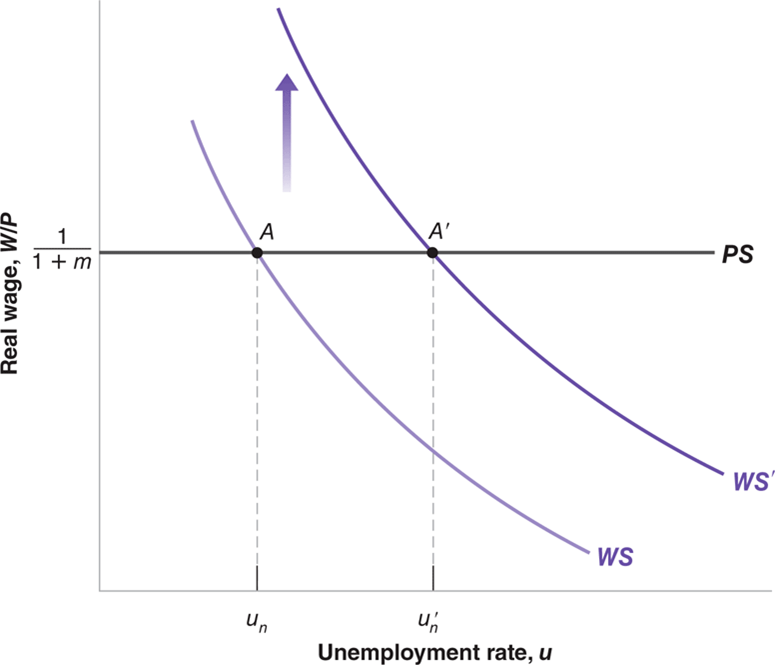
\includegraphics[scale=0.72]{graphs/L5F2.png}}
\end{frame}

\begin{frame}
\makebox[\linewidth][c]{
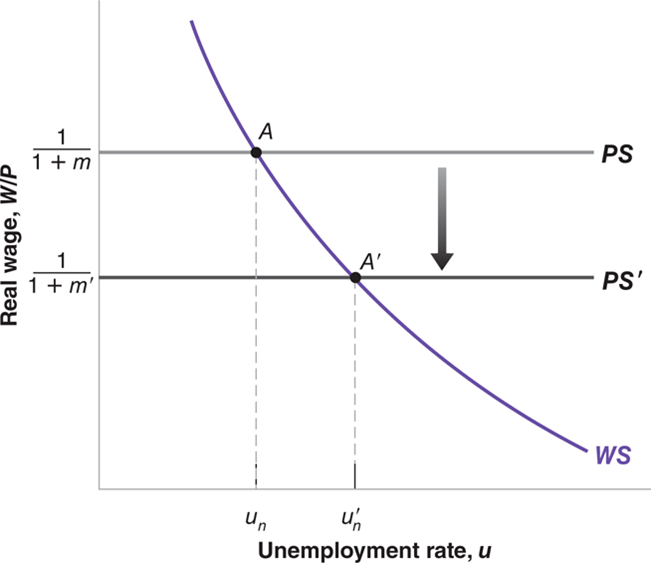
\includegraphics[scale=0.69]{graphs/L5F3.png}}
\end{frame}

\section{Unemployment, Employment,and Output}
\begin{frame}{Some Definitions}
Unemployment ($u$) is given by
\[ u = \frac{U}{L} \]
\pause
\[ u = \frac{L - N}{L} = 1 - \frac{N}{L} \]
\pause
\[ N = L(1 - u) \]
We define natural rate of employment as 
\[ N_n = L(1 - u_n) \]
\pause
We assign natural rate of output as
\[ Y_n = N_n = L(1 - u_n) \]

\end{frame}
\end{document}